\section{Results of study A}
\label{sec:results}

\subsection{Drag of the nose}

\begin{figure}[H]
\centering
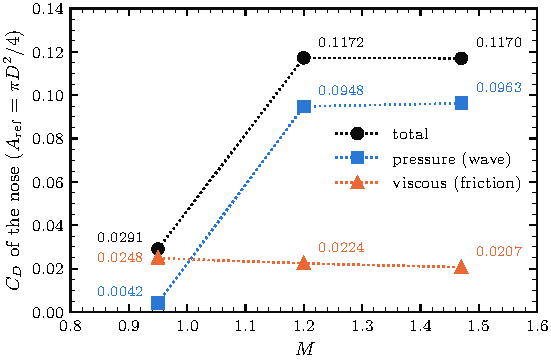
\includegraphics[width=0.62\linewidth]{fig_cd_mach}
\caption{Drag coefficient of the nose (\zone{wall\_nose}) against Mach: pressure (wave), viscous and total.
Drawn from the Fluent force reports of the three runs (Fluent cannot plot across separate runs); the
dotted lines only join the three runs.}
\label{fig:cdmach}
\end{figure}

\begin{itemize}
\item \textbf{Supersonic.} The pressure part is 0.095--0.096, 81--82\,\% of the total, and nearly
constant between $M = 1.2$ and 1.47.
\item \textbf{Transonic.} The pressure part is only 0.0042: the overpressure at the tip is almost
cancelled by the suction on the rear of the nose. Friction is 85\,\% of the total.
\item \textbf{Friction} falls from 0.0248 to 0.0207 as $\mathrm{Re}_x$ rises and the wall gets hotter.
\end{itemize}

\subsection{Flow field}

\begin{figure}[H]
\centering
\begin{subfigure}[t]{0.32\linewidth}
\centering
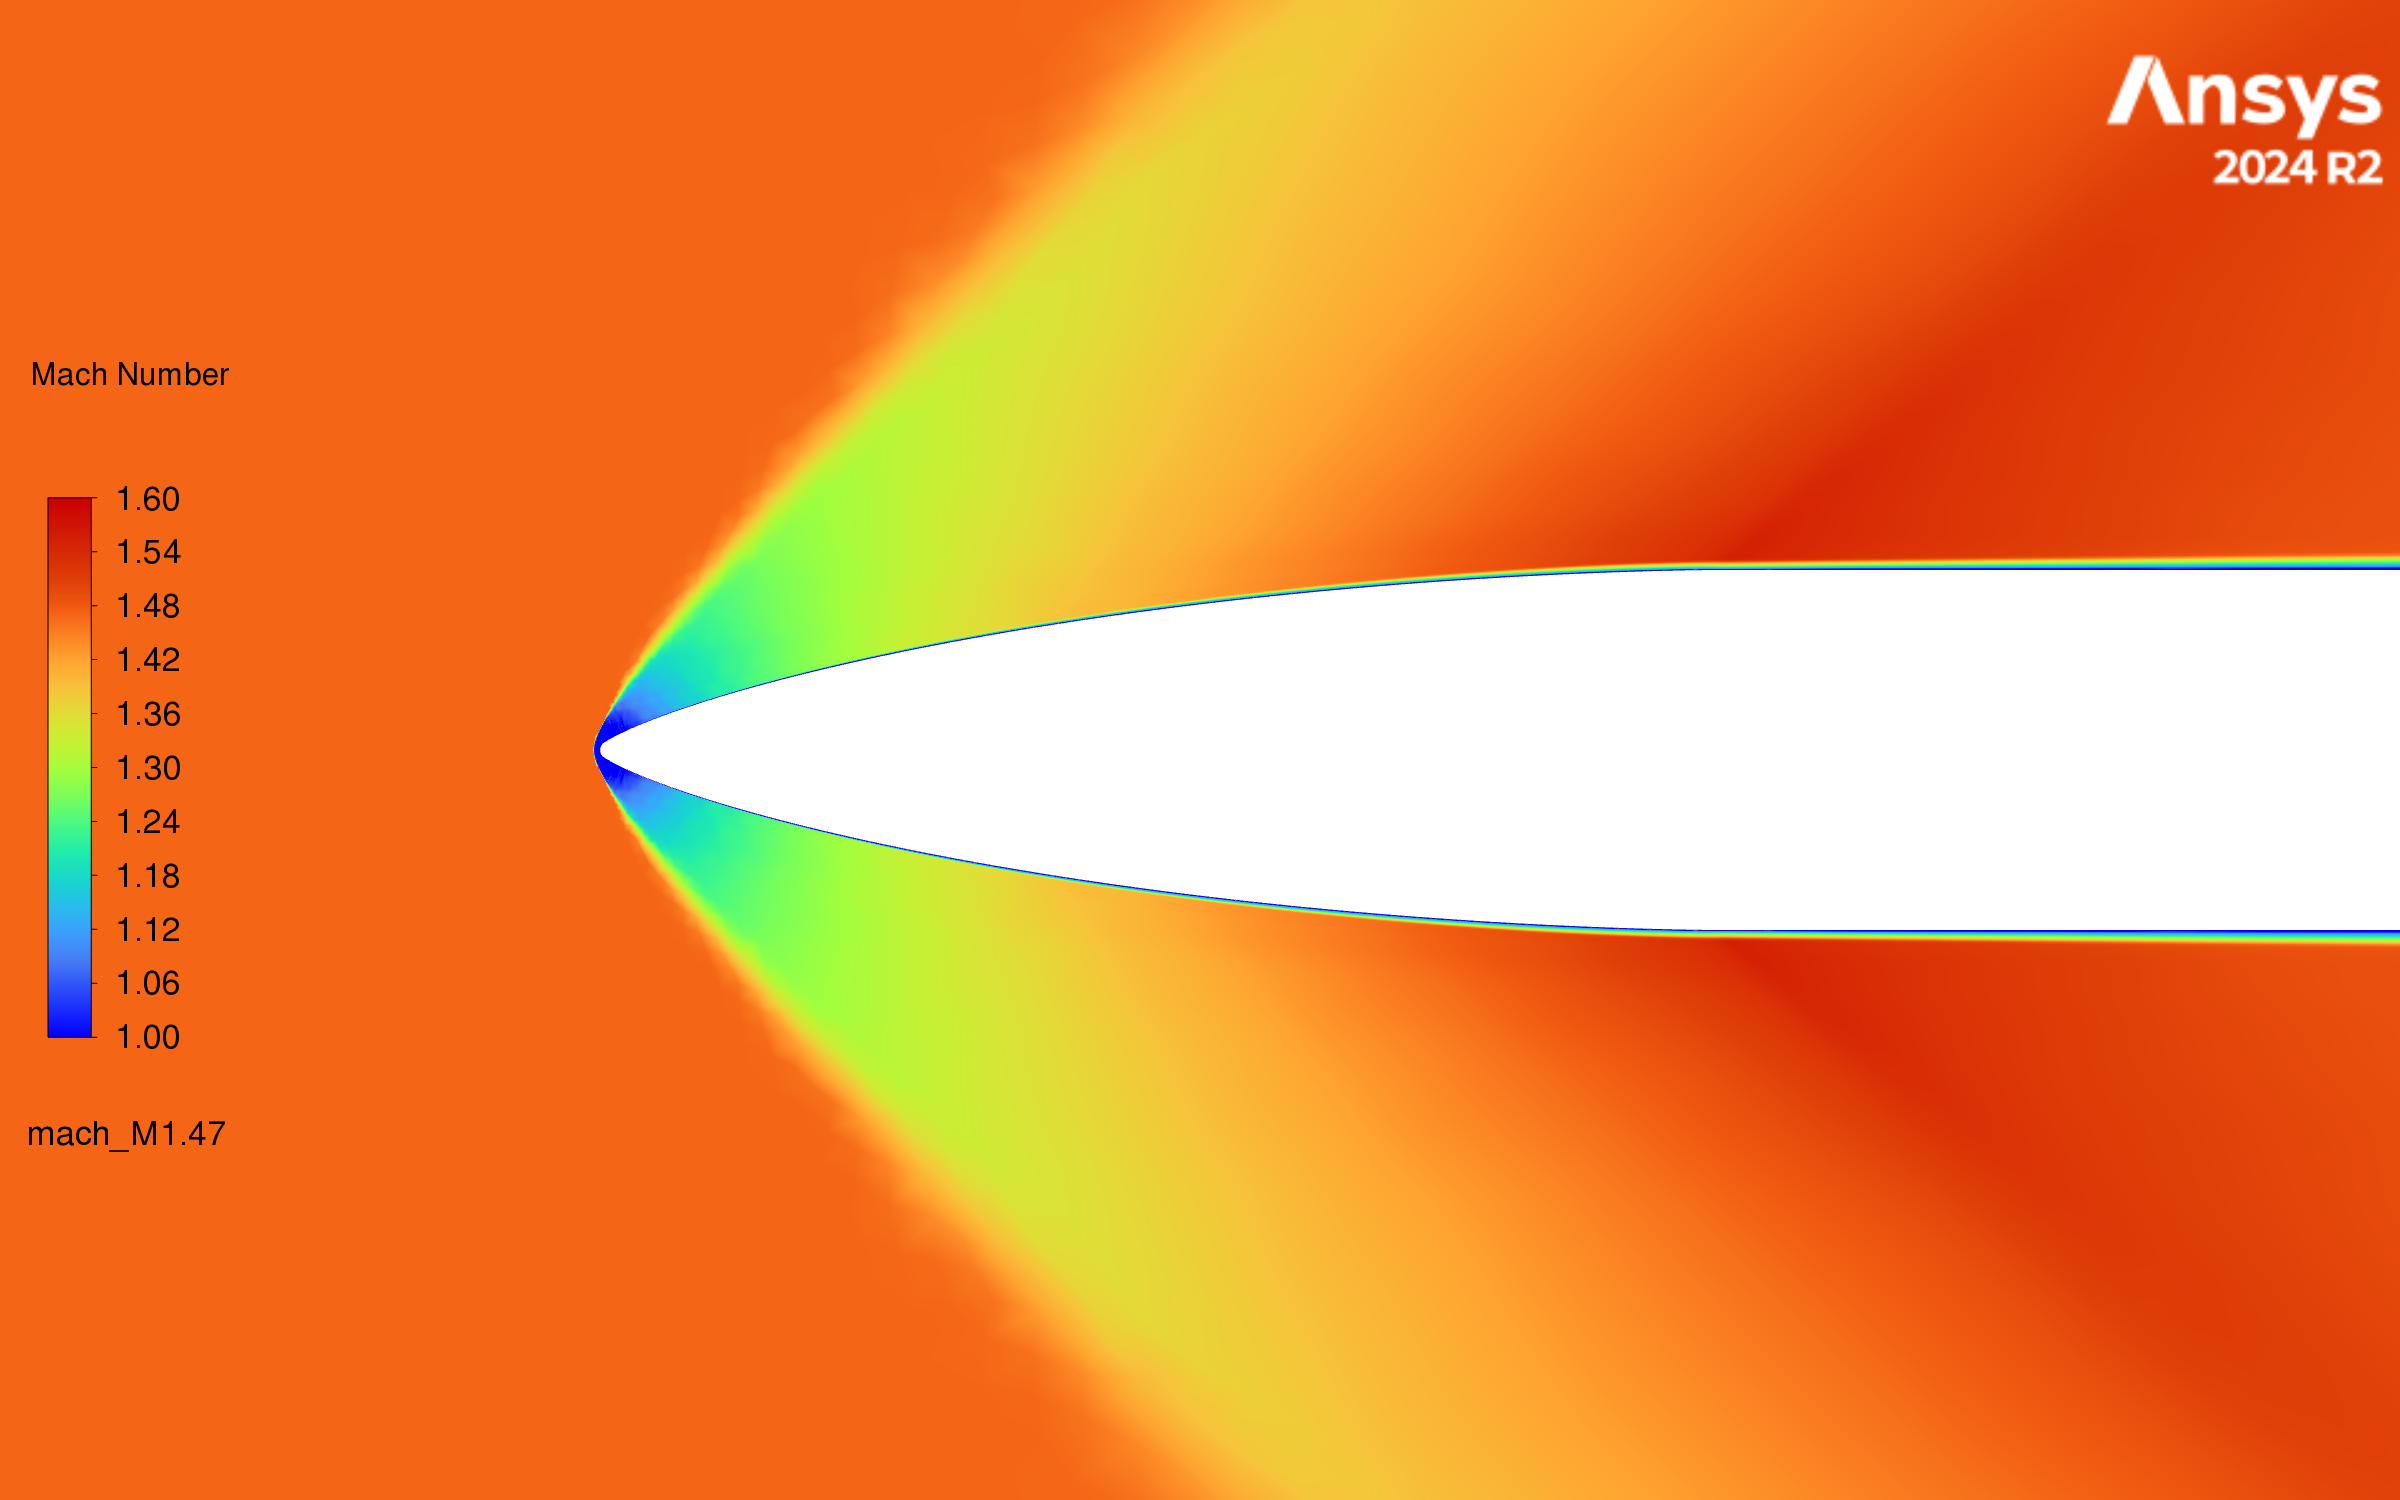
\includegraphics[width=\linewidth]{fluent_mach_M1.47}
\caption{$M = 1.47$ (1.0--1.6).}
\end{subfigure}\hfill
\begin{subfigure}[t]{0.32\linewidth}
\centering
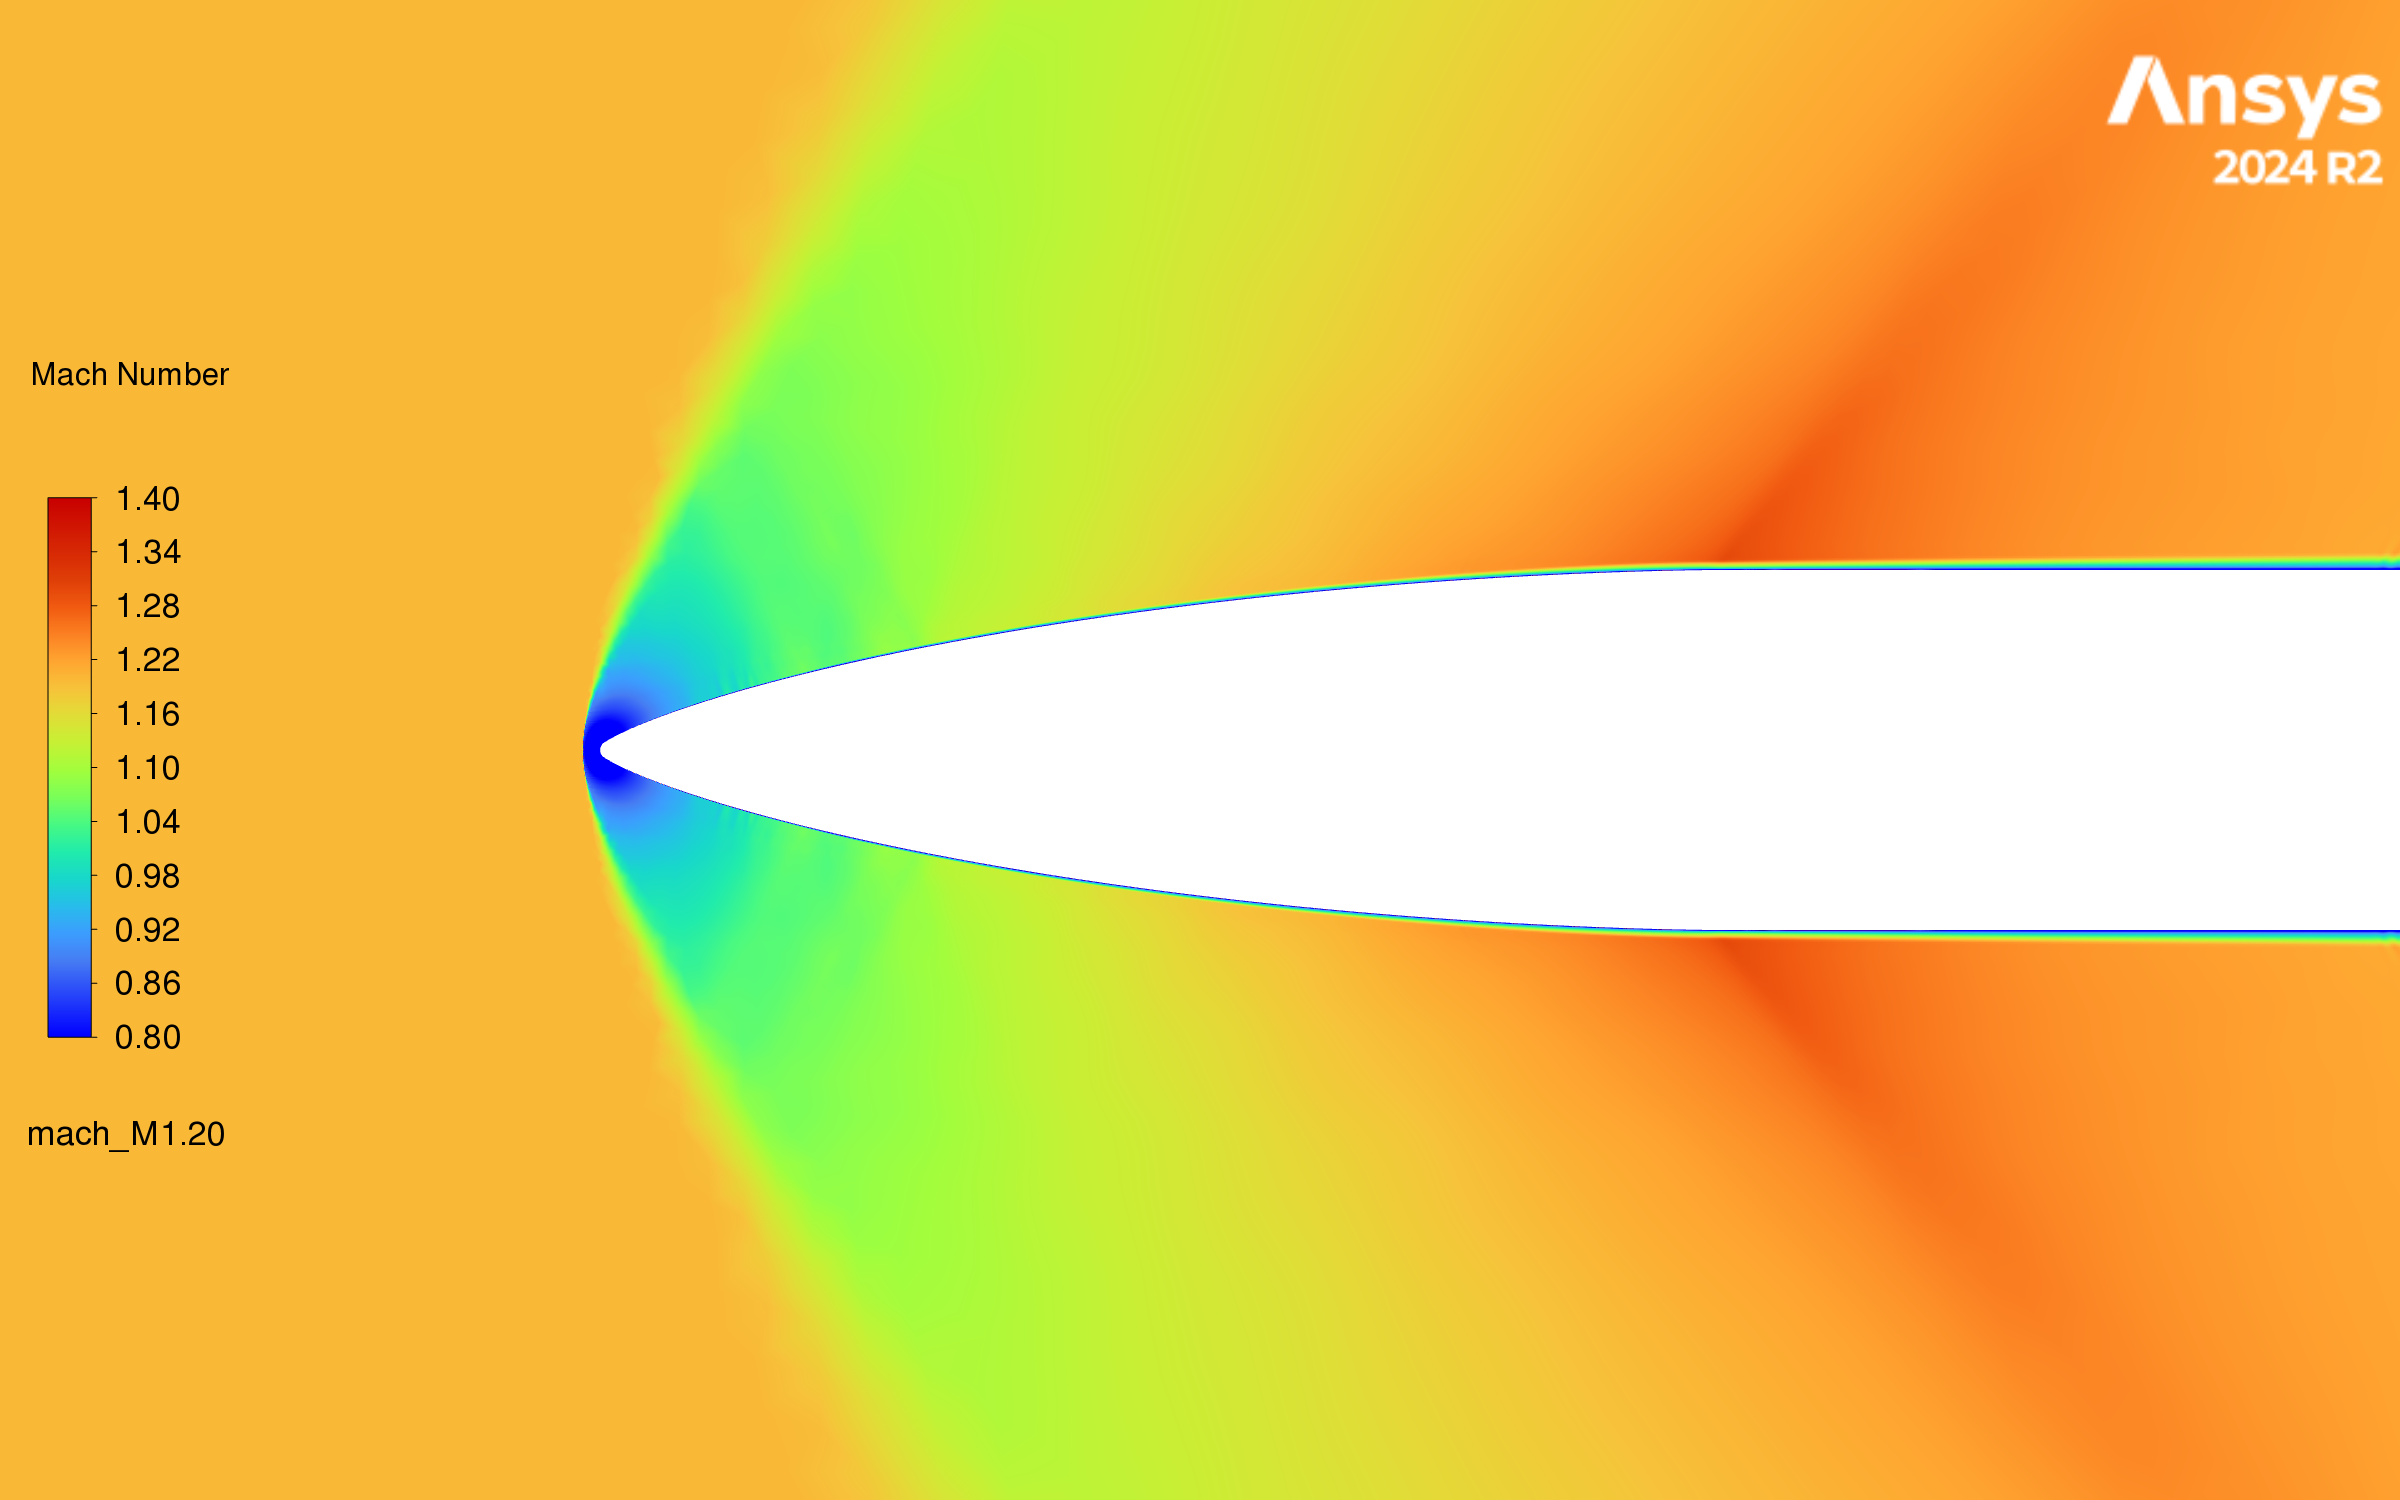
\includegraphics[width=\linewidth]{fluent_mach_M1.20}
\caption{$M = 1.2$ (0.8--1.4).}
\end{subfigure}\hfill
\begin{subfigure}[t]{0.32\linewidth}
\centering
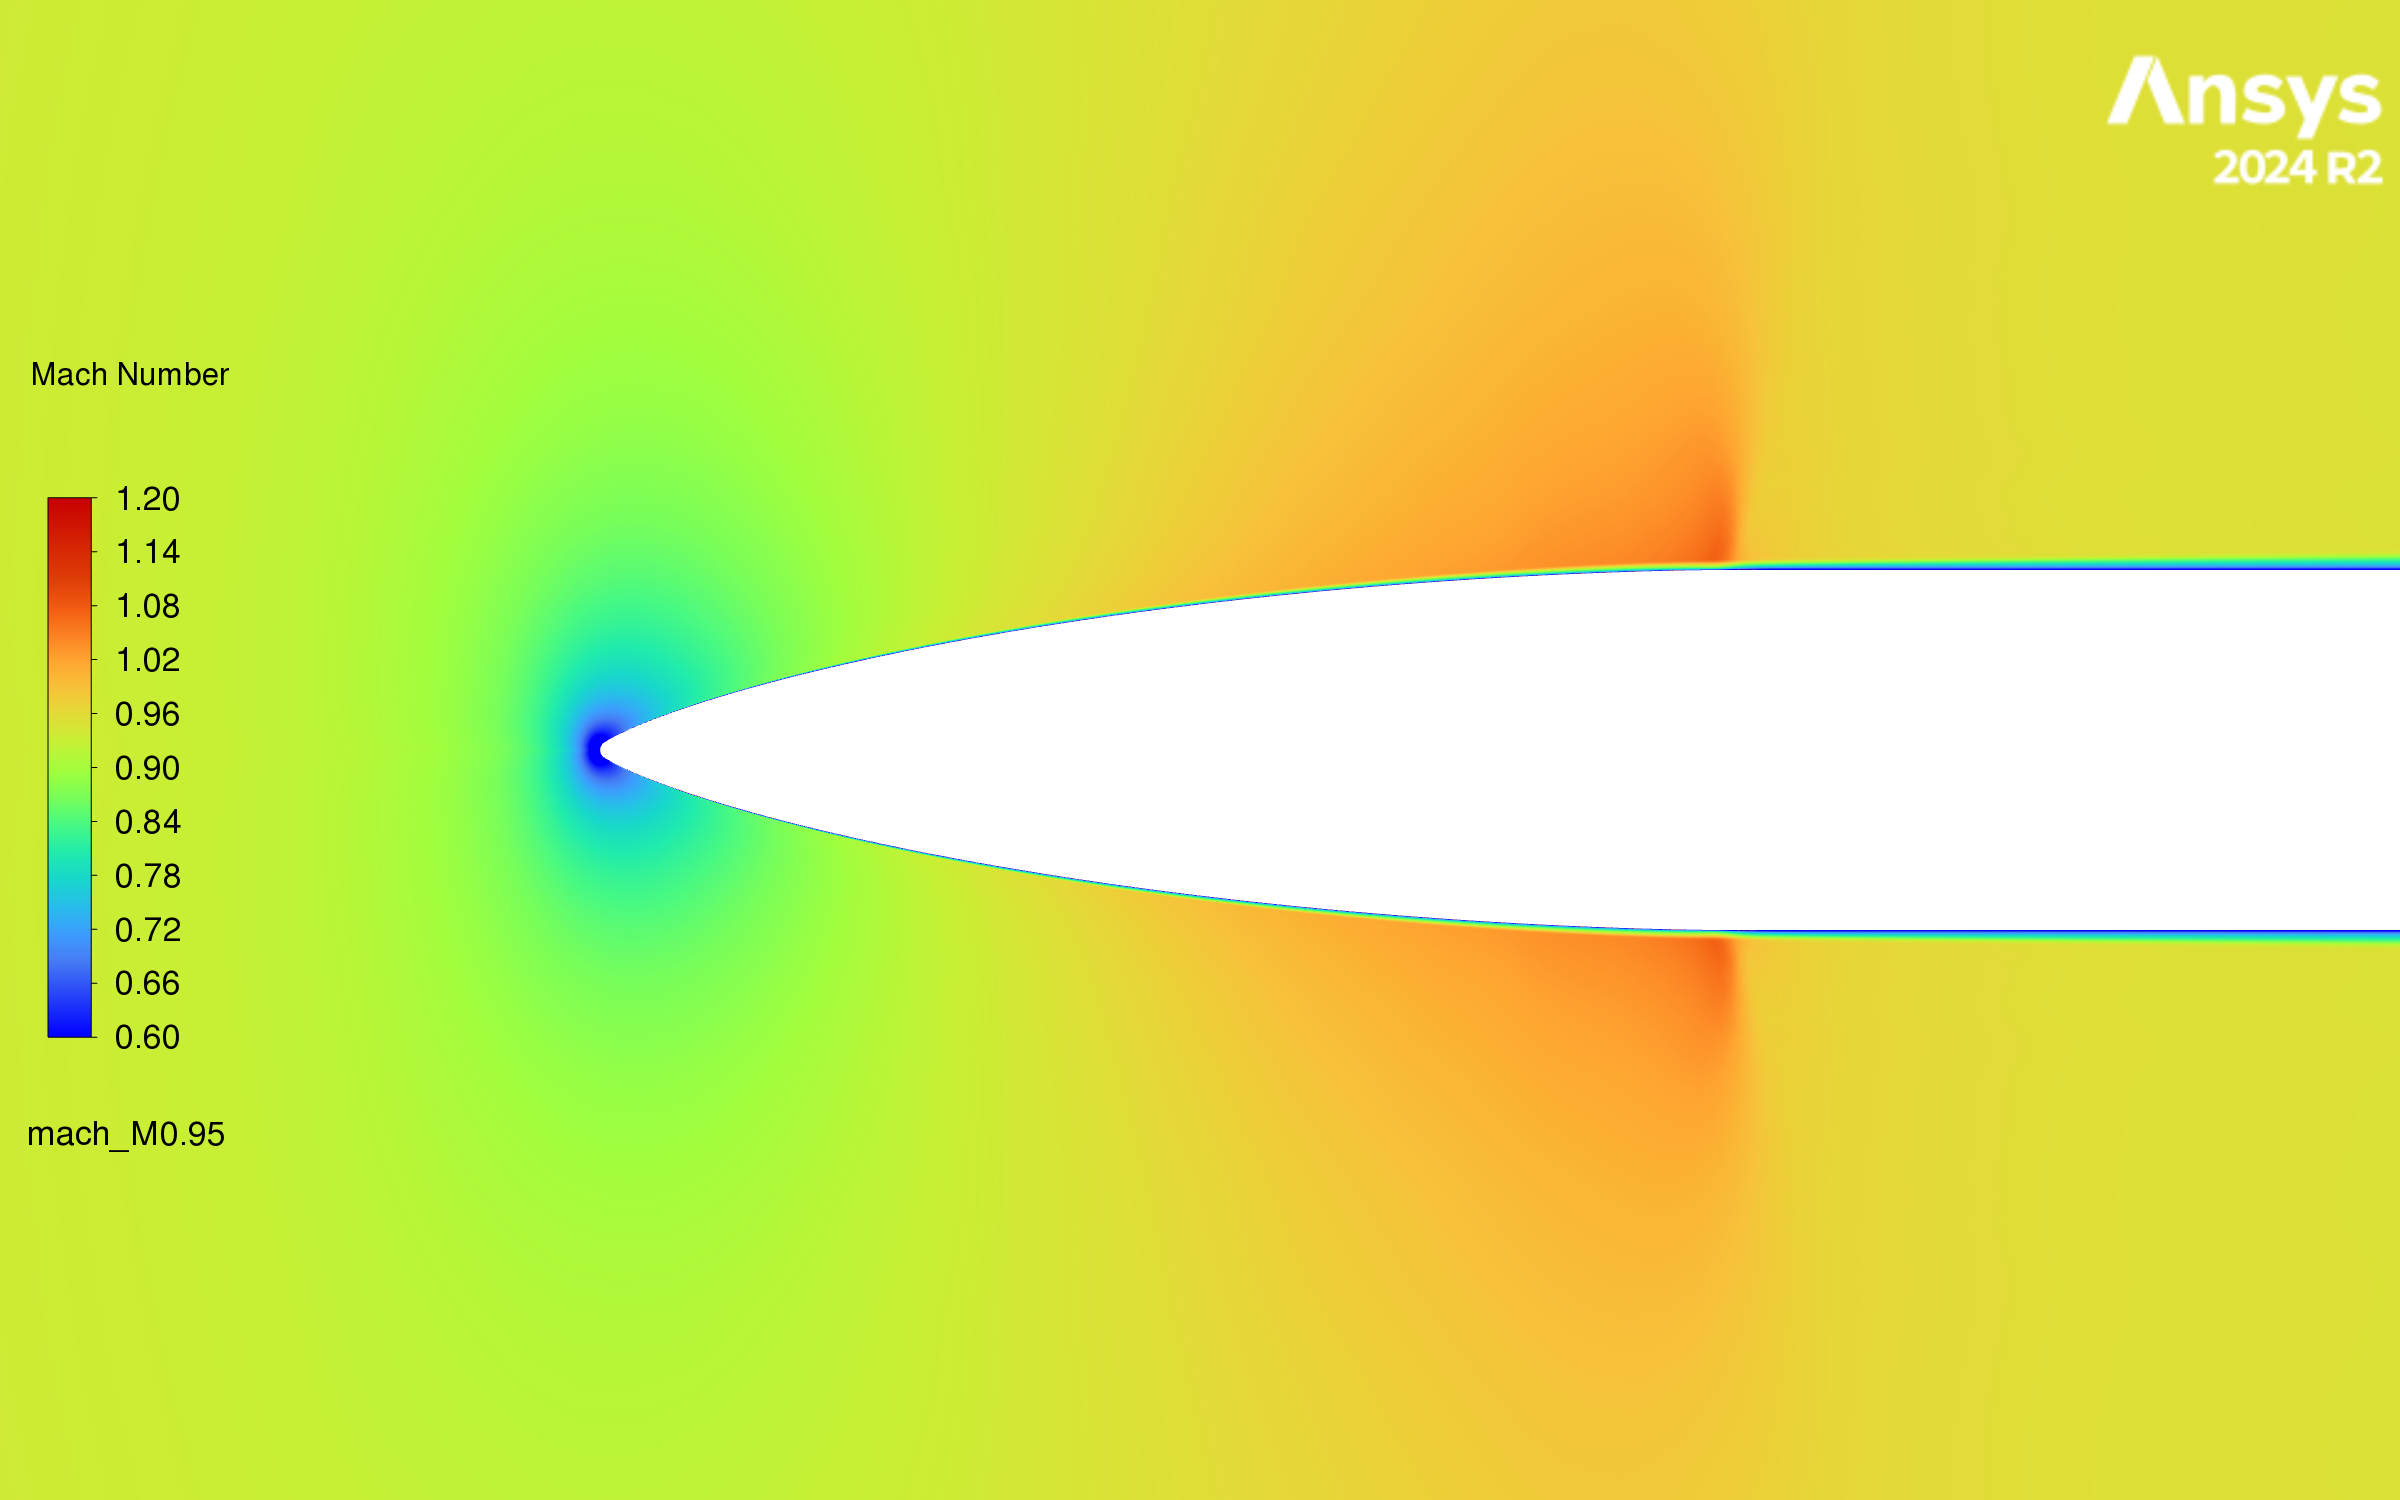
\includegraphics[width=\linewidth]{fluent_mach_M0.95}
\caption{$M = 0.95$ (0.6--1.2).}
\end{subfigure}
\caption{Mach number contours from Fluent around the nose, mirrored about the axis; each run has its own
colour scale.}
\label{fig:mach}
\end{figure}

\begin{itemize}
\item \textbf{$M = 1.47$.} The bow shock stands off the blunt tip, with subsonic flow behind it near the
axis (dark blue). It weakens outwards to $M \approx 1.3$--1.4. The flow re-expands along the nose to
$M \approx 1.55$ at the shoulder.
\item \textbf{$M = 1.2$.} Same picture; the shock stands further off and is more curved. $M \approx 1.3$
at the shoulder.
\item \textbf{$M = 0.95$.} No bow shock. The flow stagnates at the tip and accelerates along the nose; a
supersonic pocket ($M \approx 1.05$--1.1) forms at the shoulder and ends in a weak shock.
\end{itemize}

\begin{figure}[H]
\centering
\begin{subfigure}[t]{0.32\linewidth}
\centering
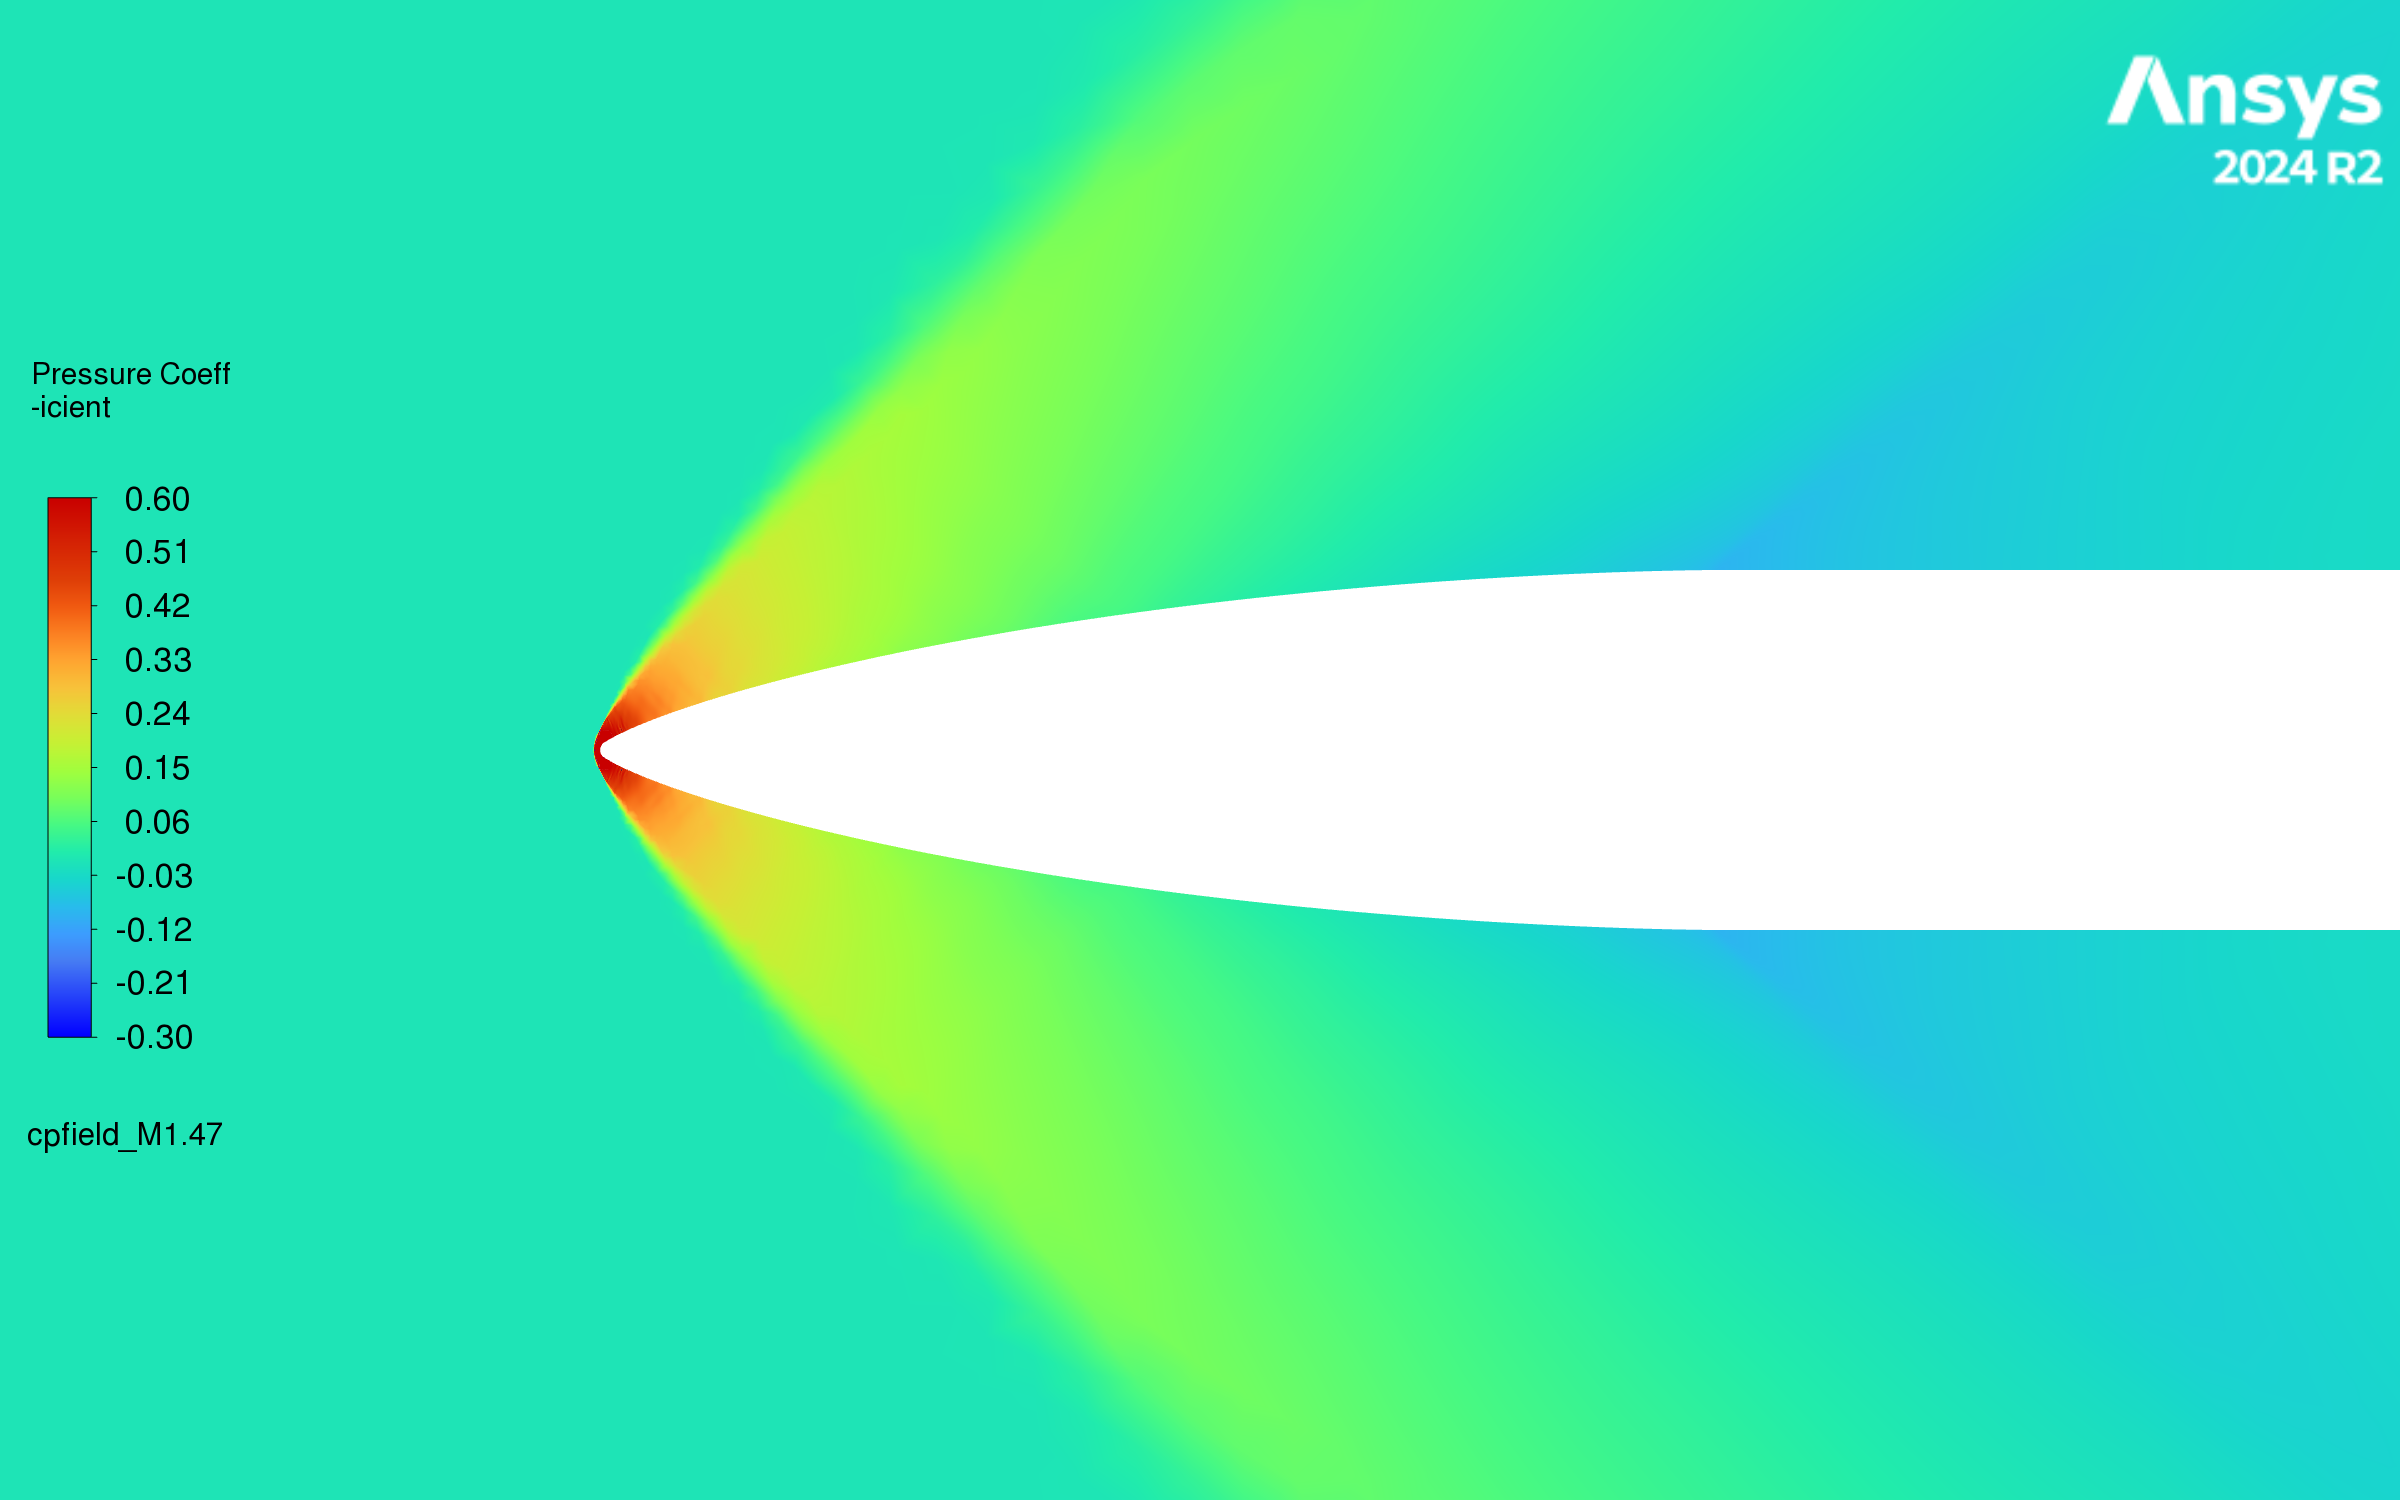
\includegraphics[width=\linewidth]{fluent_cpfield_M1.47}
\caption{$M = 1.47$.}
\end{subfigure}\hfill
\begin{subfigure}[t]{0.32\linewidth}
\centering
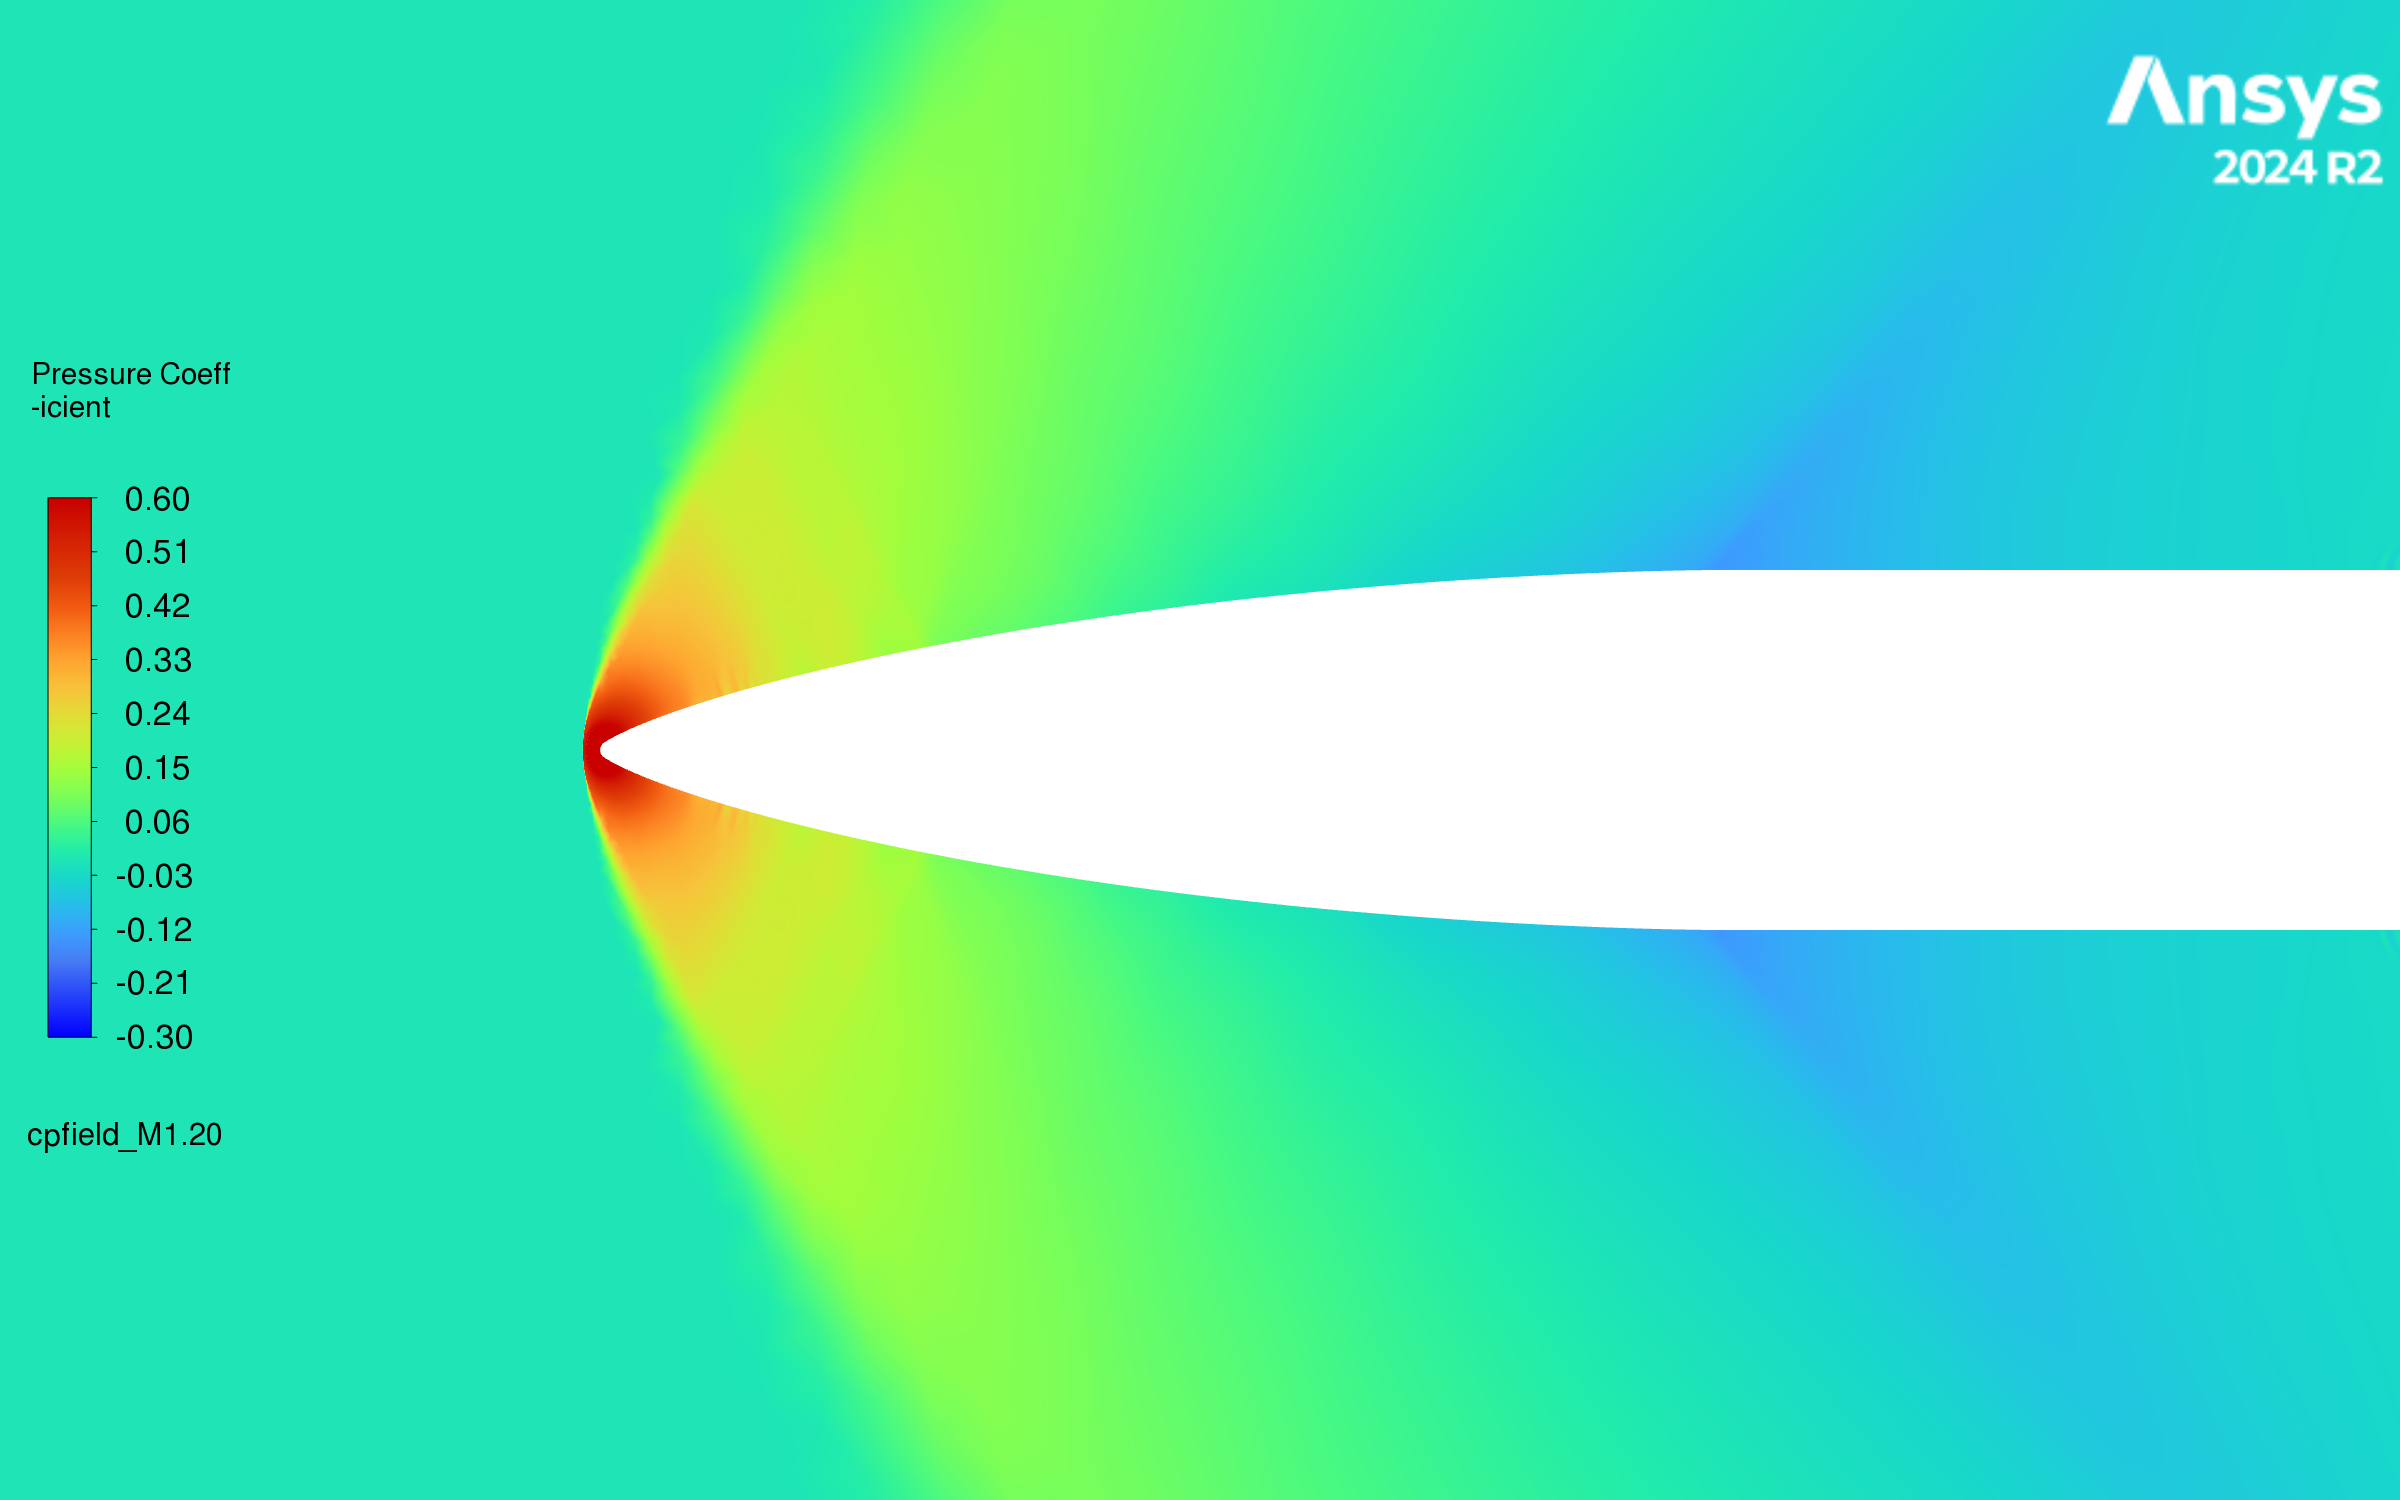
\includegraphics[width=\linewidth]{fluent_cpfield_M1.20}
\caption{$M = 1.2$.}
\end{subfigure}\hfill
\begin{subfigure}[t]{0.32\linewidth}
\centering
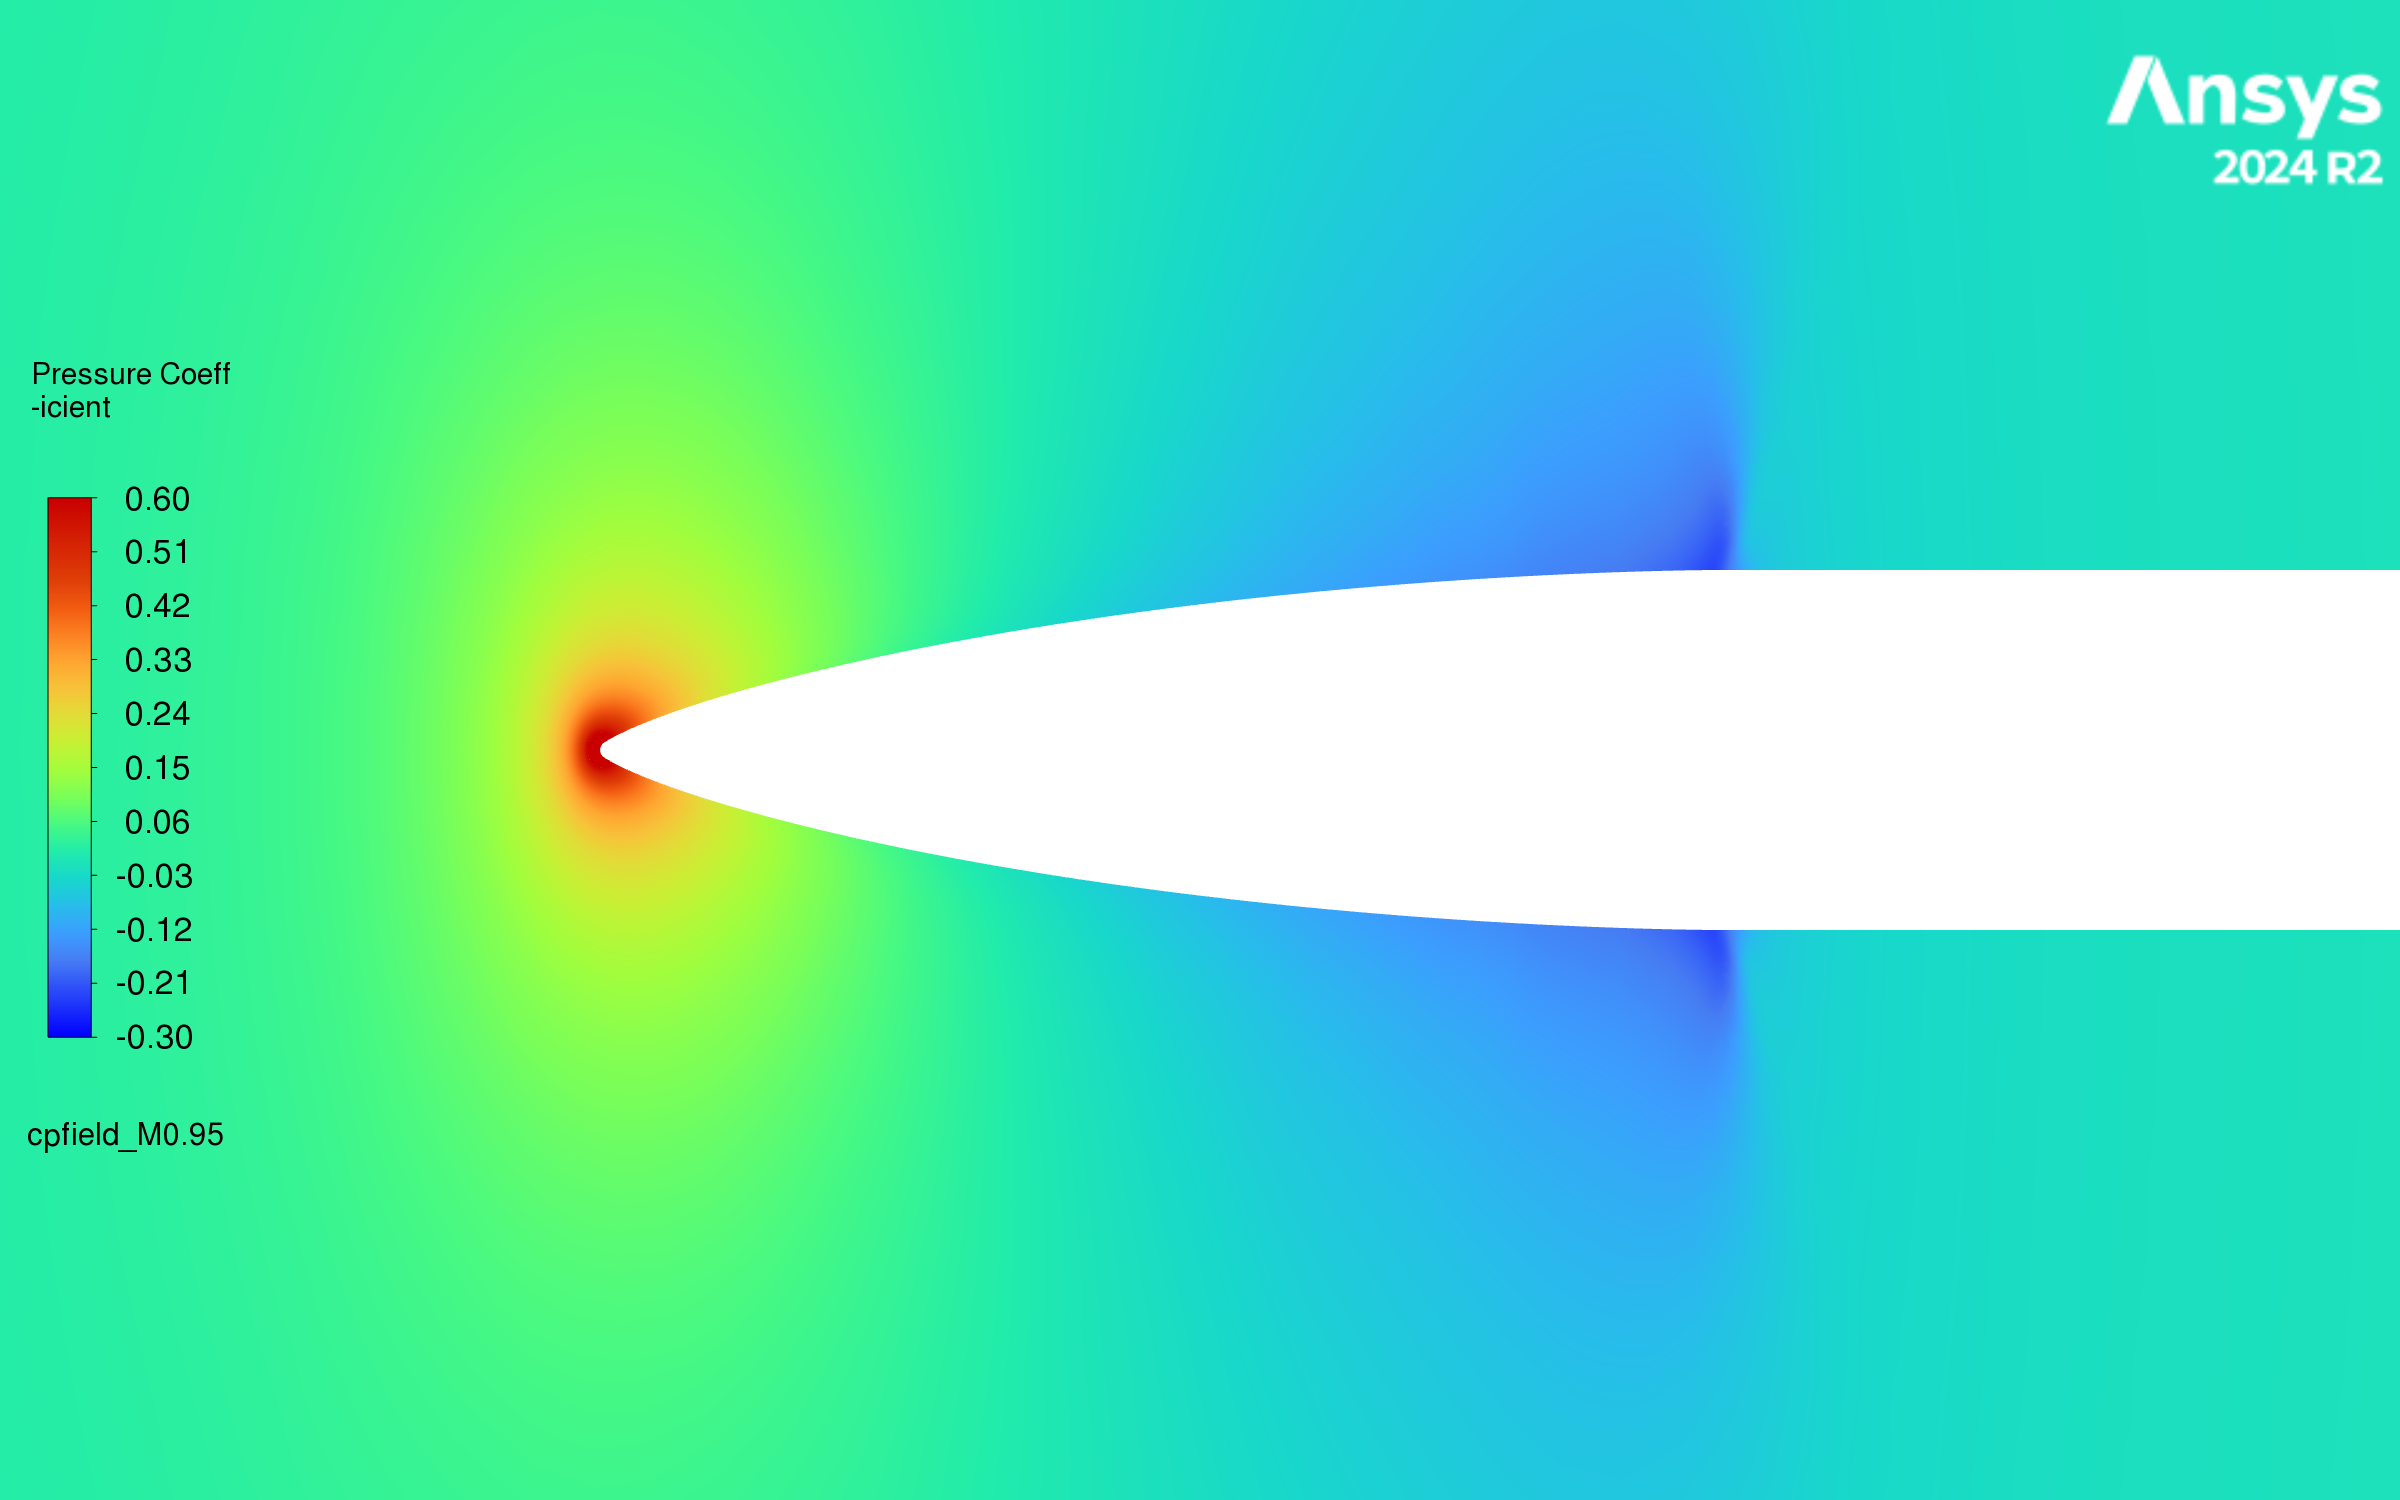
\includegraphics[width=\linewidth]{fluent_cpfield_M0.95}
\caption{$M = 0.95$.}
\end{subfigure}
\caption{Pressure coefficient $C_p = (p - p_\infty)/q_\infty$ around the nose, from Fluent, on the same
colour scale ($-0.3$ to 0.6) for all three runs.}
\label{fig:cpfield}
\end{figure}

Above $M = 1$ the high pressure behind the bow shock (red to yellow) covers the front half of the nose:
that is the wave drag. At $M = 0.95$ the high pressure stays close to the tip and the rear of the nose is
in suction (blue), so the two nearly cancel (Figure~\ref{fig:cpfield}).

\subsection{Checks}

\begin{table}[H]
\centering
\caption{Checks of the three runs.}
\label{tab:checks}
\small
\begin{tabular}{@{}lrrr@{}}
\toprule
 & $M = 0.95$ & $M = 1.2$ & $M = 1.47$ \\
\midrule
Maximum $y^+$ on \zone{wall\_nose} / \zone{wall\_body} & 0.51 / 0.28 & 0.60 / 0.30 & 0.71 / 0.29 \\
Drag force $F_x$ on \zone{wall\_nose} & \SI{42.32}{N} & \SI{254.75}{N} & \SI{349.42}{N} \\
\texttt{cd-nose} reported by Fluent & 0.0291 & 0.1172 & 0.1170 \\
$\Delta$ over the last 500 iterations & 0.009\,\% & 0.083\,\% & 0.032\,\% \\
\bottomrule
\end{tabular}
\end{table}

\begin{itemize}
\item $y^+ < 1$ on both walls at all three Mach numbers.
\item Not done yet: a mesh-independence study (Section~\ref{sec:conclusions}).
\end{itemize}

\subsection{Pressure and friction along the nose}

\begin{figure}[H]
\centering
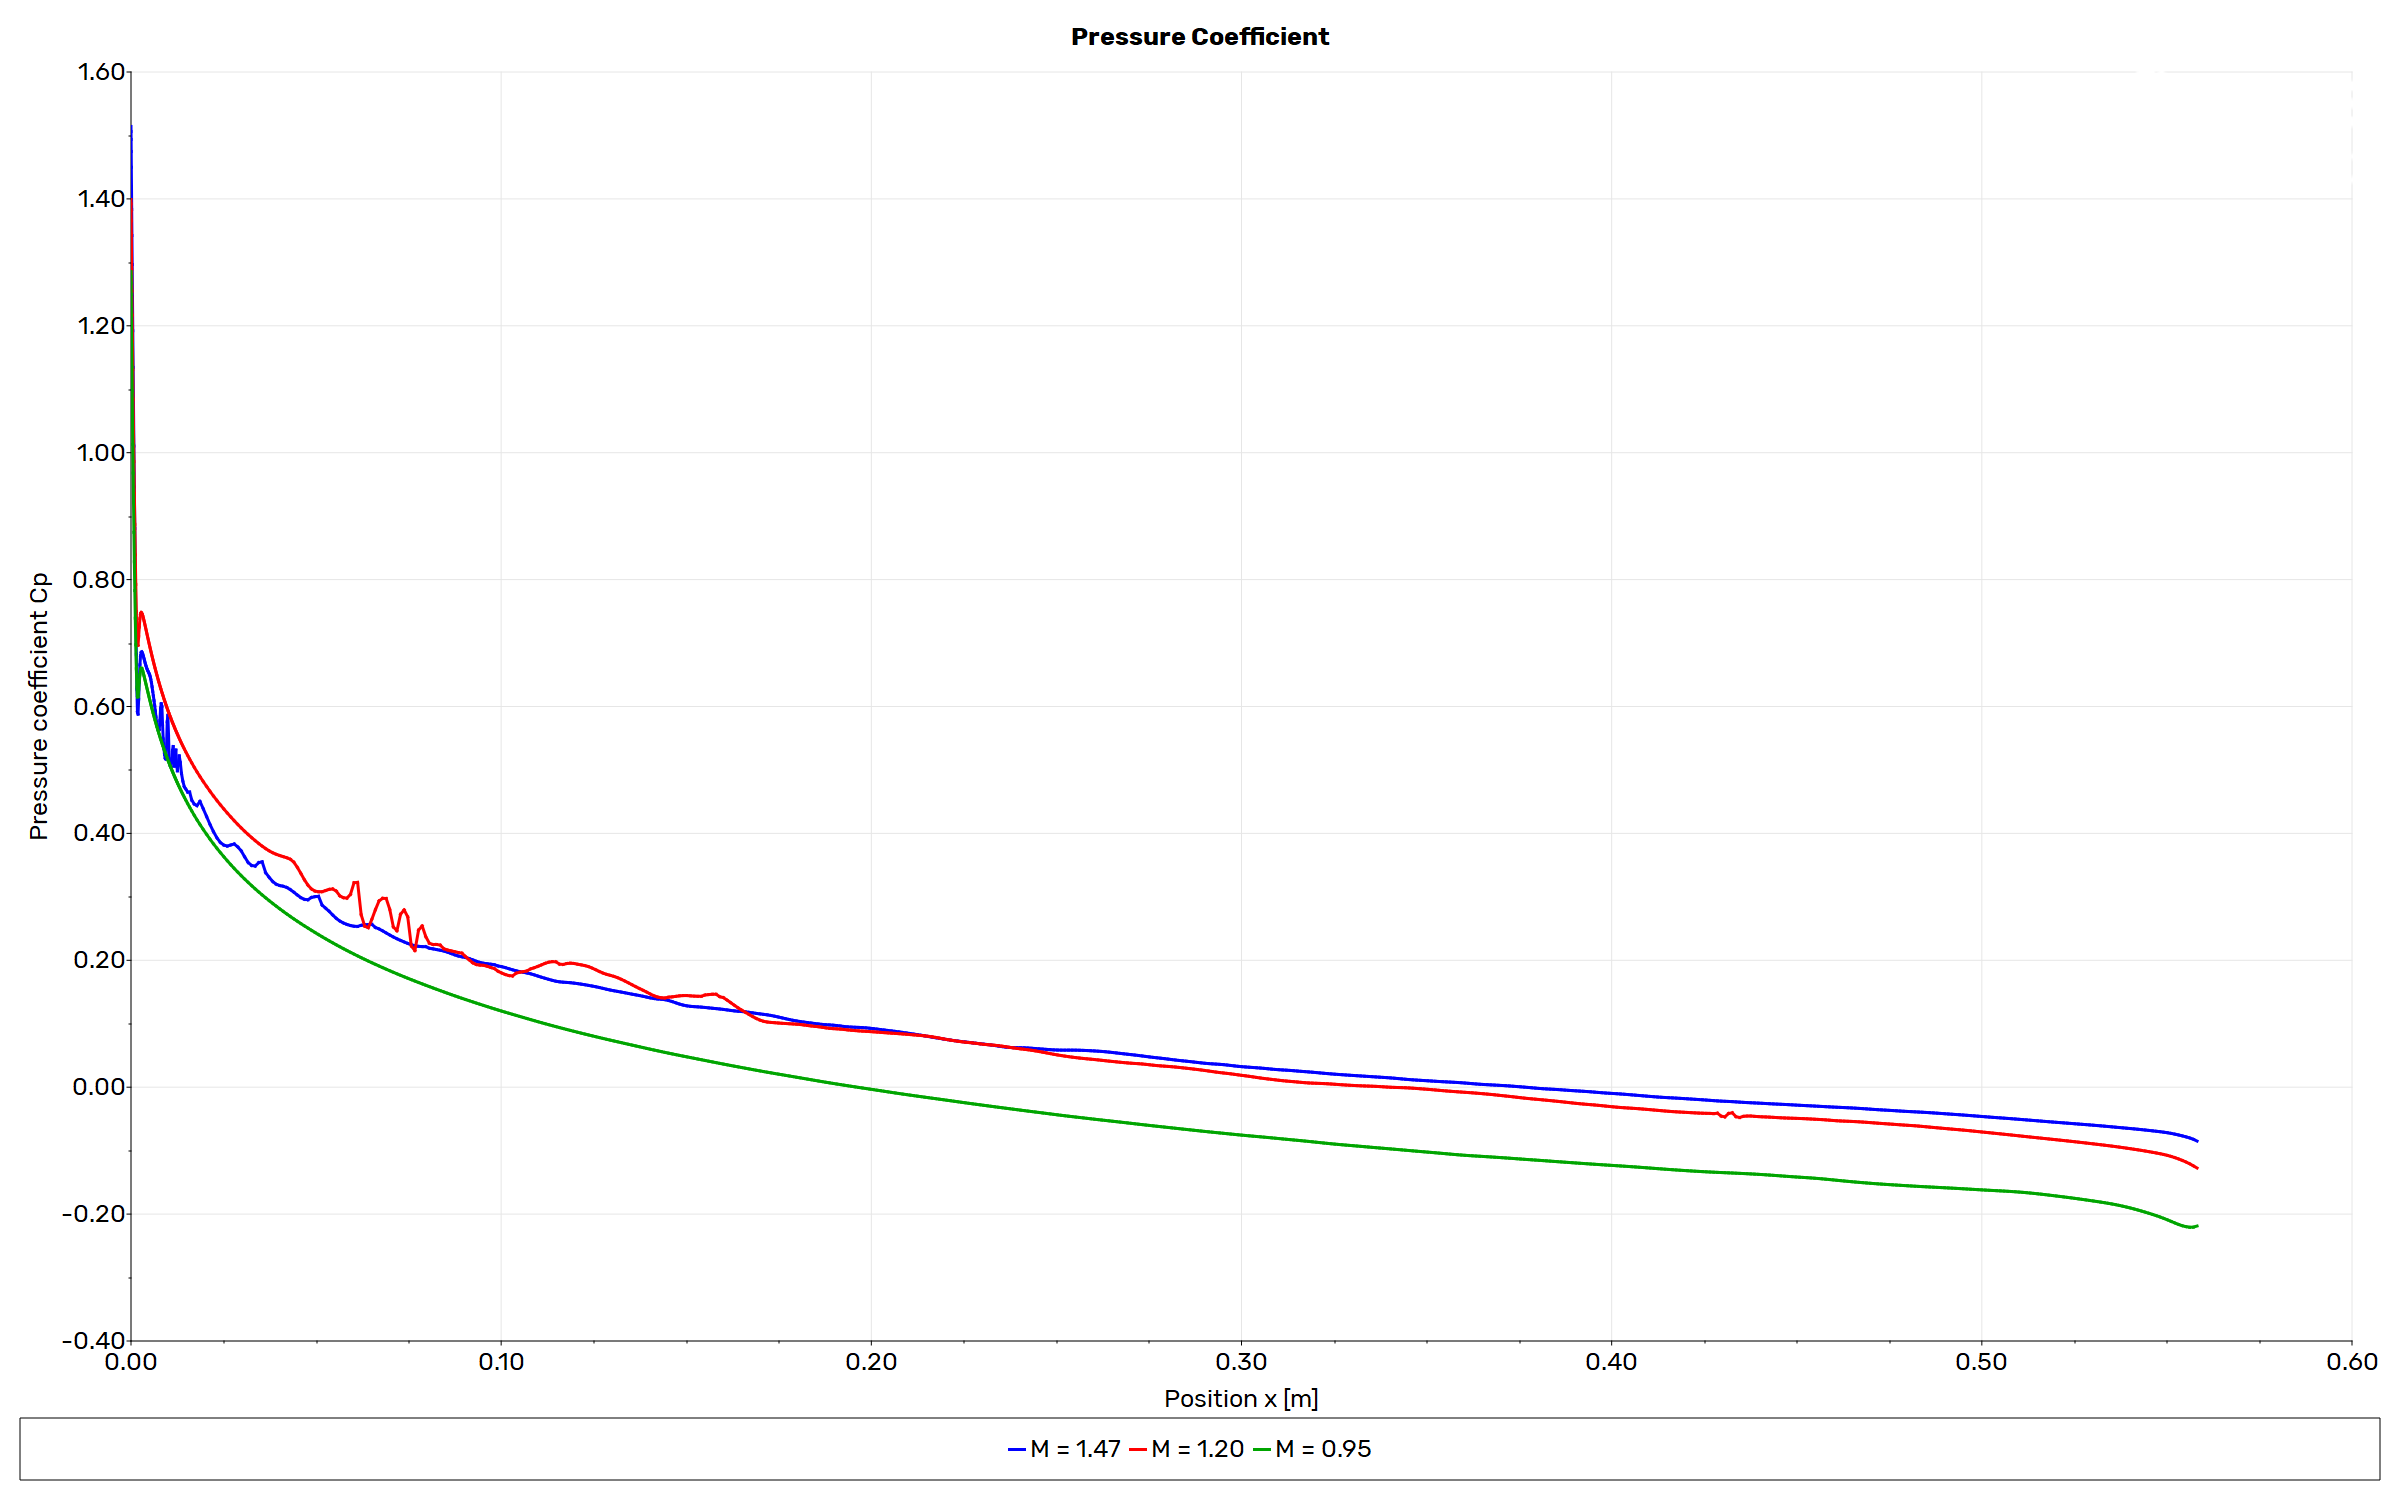
\includegraphics[width=0.9\linewidth]{fluent_cp_all}
\caption{Pressure coefficient along \zone{wall\_nose} at the three Mach numbers (Fluent XY plot).}
\label{fig:cp}
\end{figure}

\begin{figure}[H]
\centering
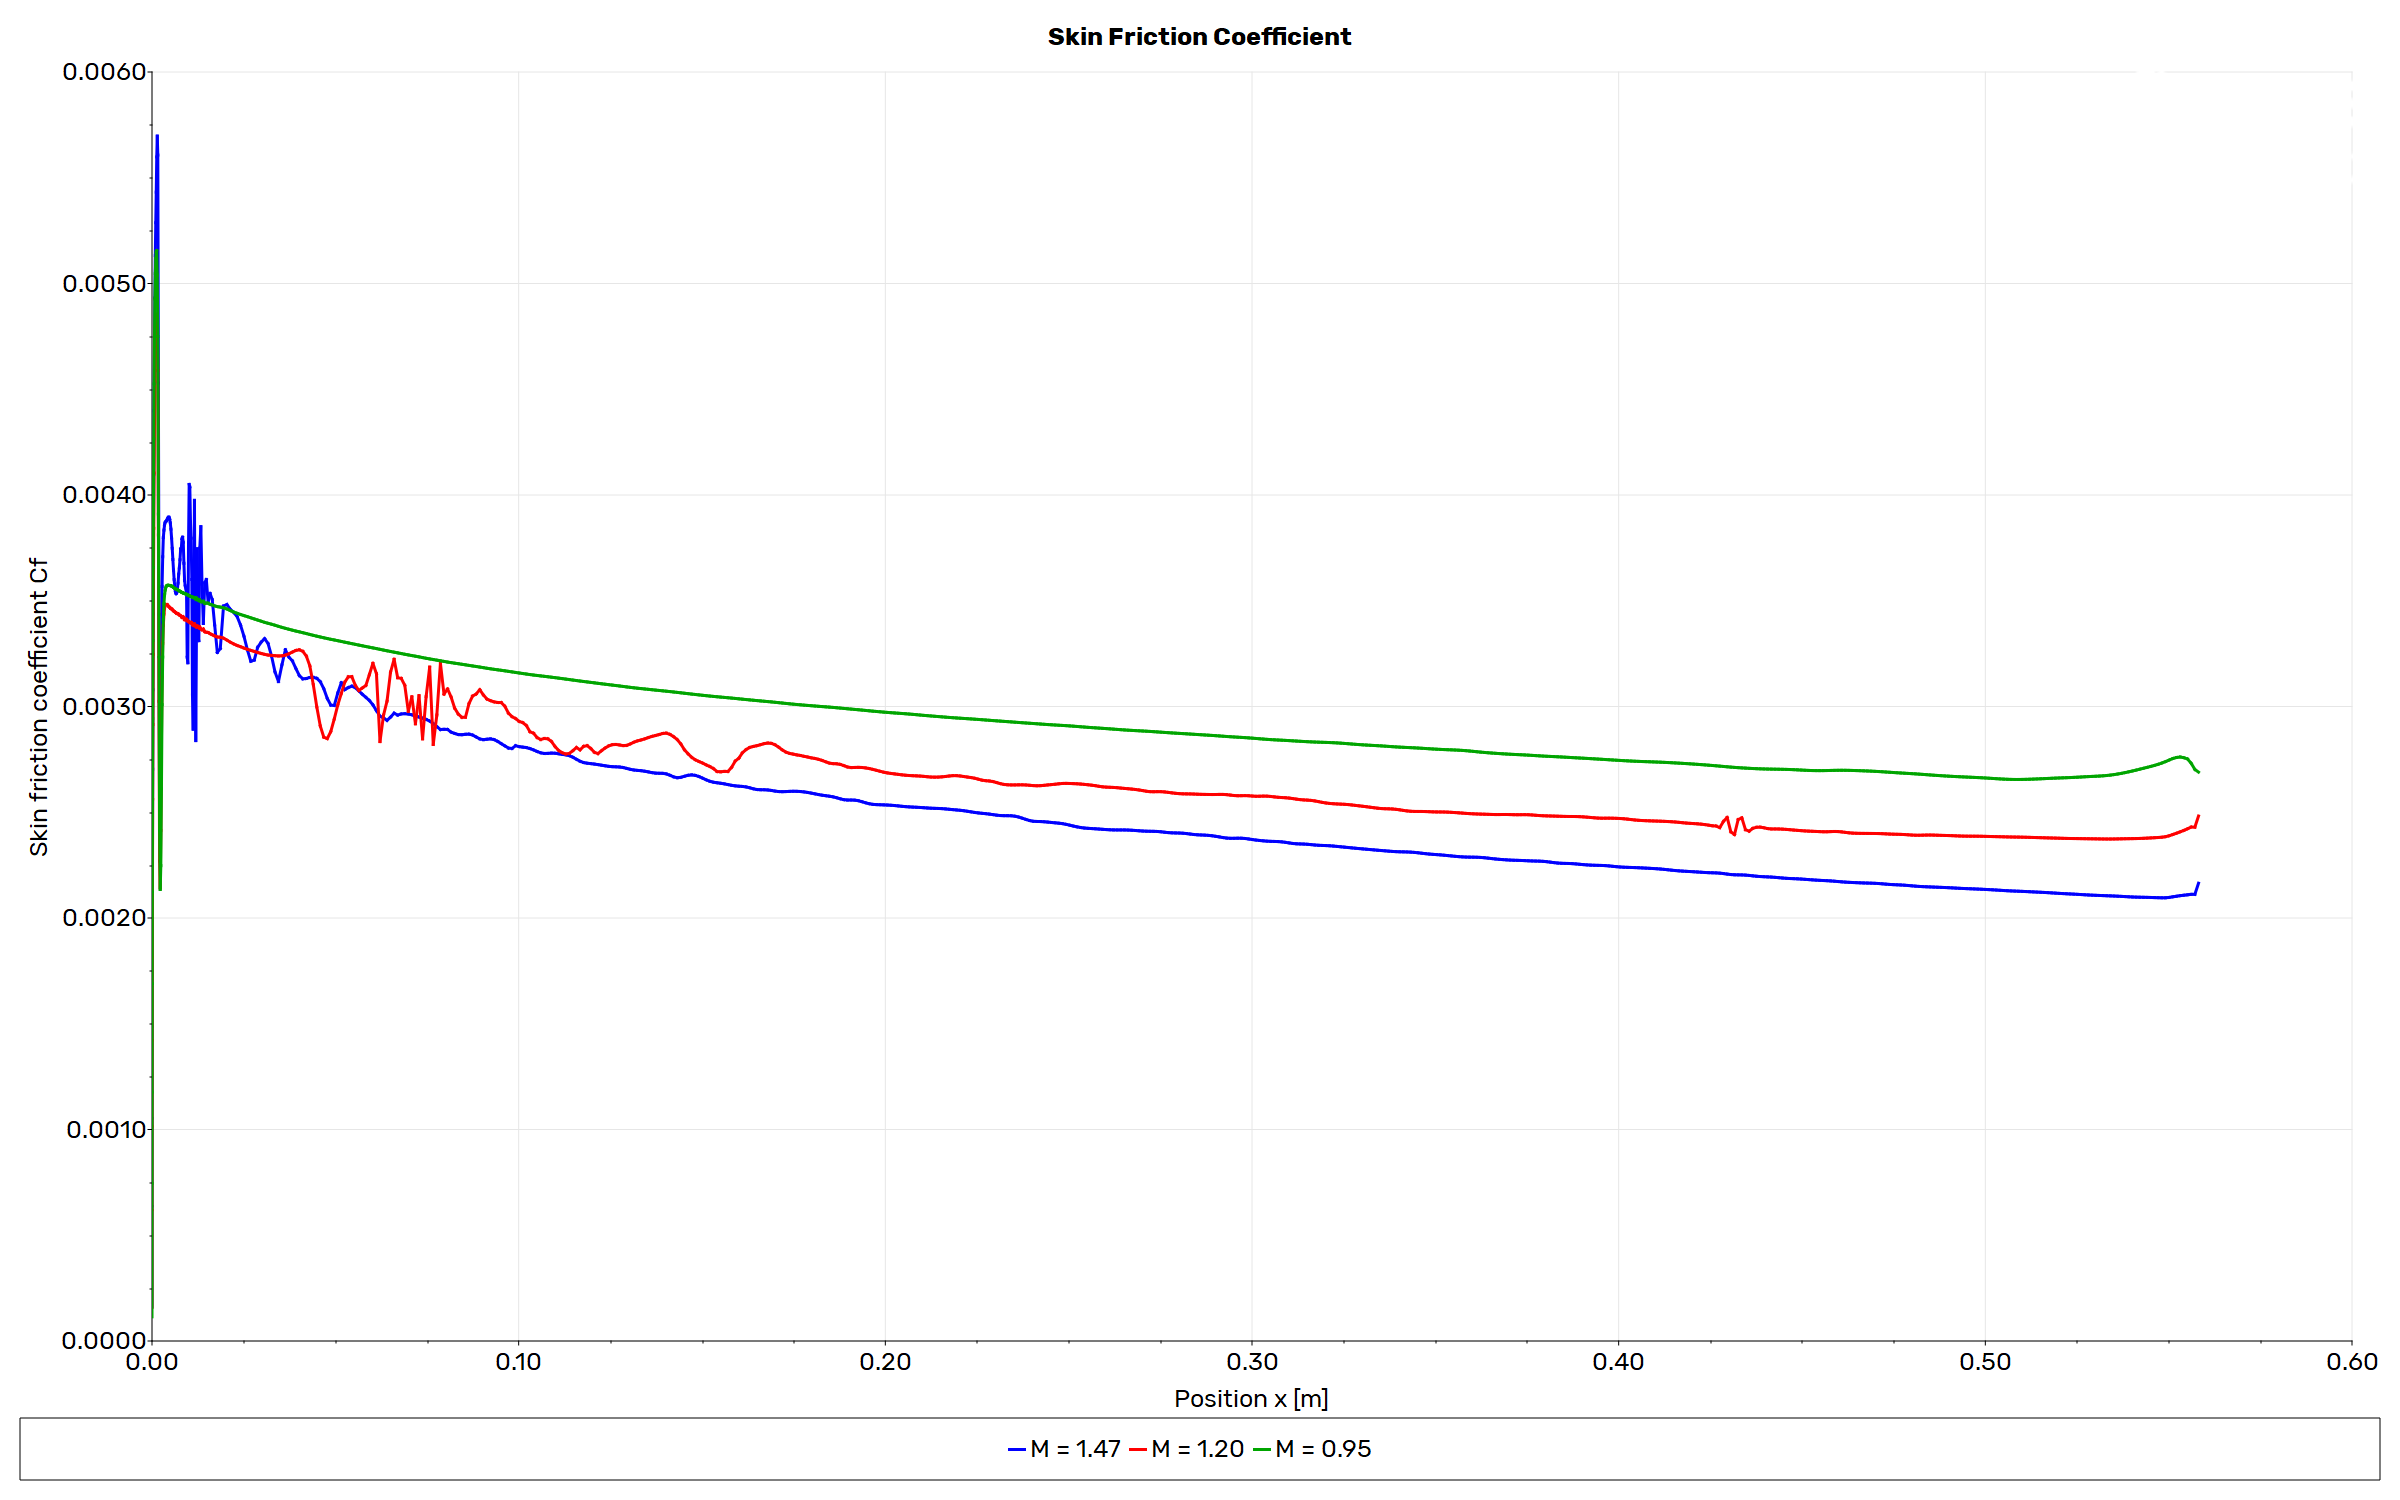
\includegraphics[width=0.9\linewidth]{fluent_cf_all}
\caption{Skin-friction coefficient along \zone{wall\_nose} at the three Mach numbers (Fluent XY plot).}
\label{fig:cf}
\end{figure}

\paragraph{Pressure (Figure~\ref{fig:cp}).} It peaks at the tip, $C_p = 1.51$ ($M = 1.47$) and 1.40
($M = 1.2$), within 0.4\,\% of the normal-shock value: the bow shock is captured correctly. Above $M = 1$
the wall stays above $p_\infty$ up to $x \approx 340$--\SI{375}{mm}: that is the wave drag. At
$M = 0.95$ it drops below $p_\infty$ at $x \approx \SI{195}{mm}$ and reaches $C_p = -0.22$ at the
shoulder, so the suction cancels most of the push on the front. The wiggles at $x = 50$--\SI{170}{mm}
($M = 1.2$) are numerical and average out.

\paragraph{Friction (Figure~\ref{fig:cf}).} Highest just behind the tip ($\approx 5\cdot10^{-3}$), it falls
to 2.2--$2.7\cdot10^{-3}$ at the shoulder as the boundary layer grows, and is lower at higher $M$.
